The Ensemble Model merges the predictions from the three models above: the ROUGE-Based Model, the LightGBM Model and the Transformer, as shown in
\hyperref[fig:ensemble-model]{Figure~\ref{fig:ensemble-model}}.
Each of these models independently predicts both content and wording scores, which the Ensemble Model combines into the two final scores.

\subsubsection{Model Architecture}

The summary, reference text, and the prompt are provided as raw text inputs for this ensemble. Each of the three individual models perform their own preprocessing steps on the texts. (These steps are explained in their respective sections above).
Following preprocessing, the models make their predictions, which the ensemble aggregates using a single linear layer, down-projecting them into the two final predictions. The linear layer is trained to predict scores based on the outputs of the three models, effectively learning how to weigh each model's contribution. Instead of a simple (weighted) average, the ensemble learns to leverage the strengths of each model: the ROUGE-Based Model performs well on the content score, LGBM on the wording score, and the Transformer is a great generalizer that also takes the specific question of the task into consideration.

\begin{figure}[H]
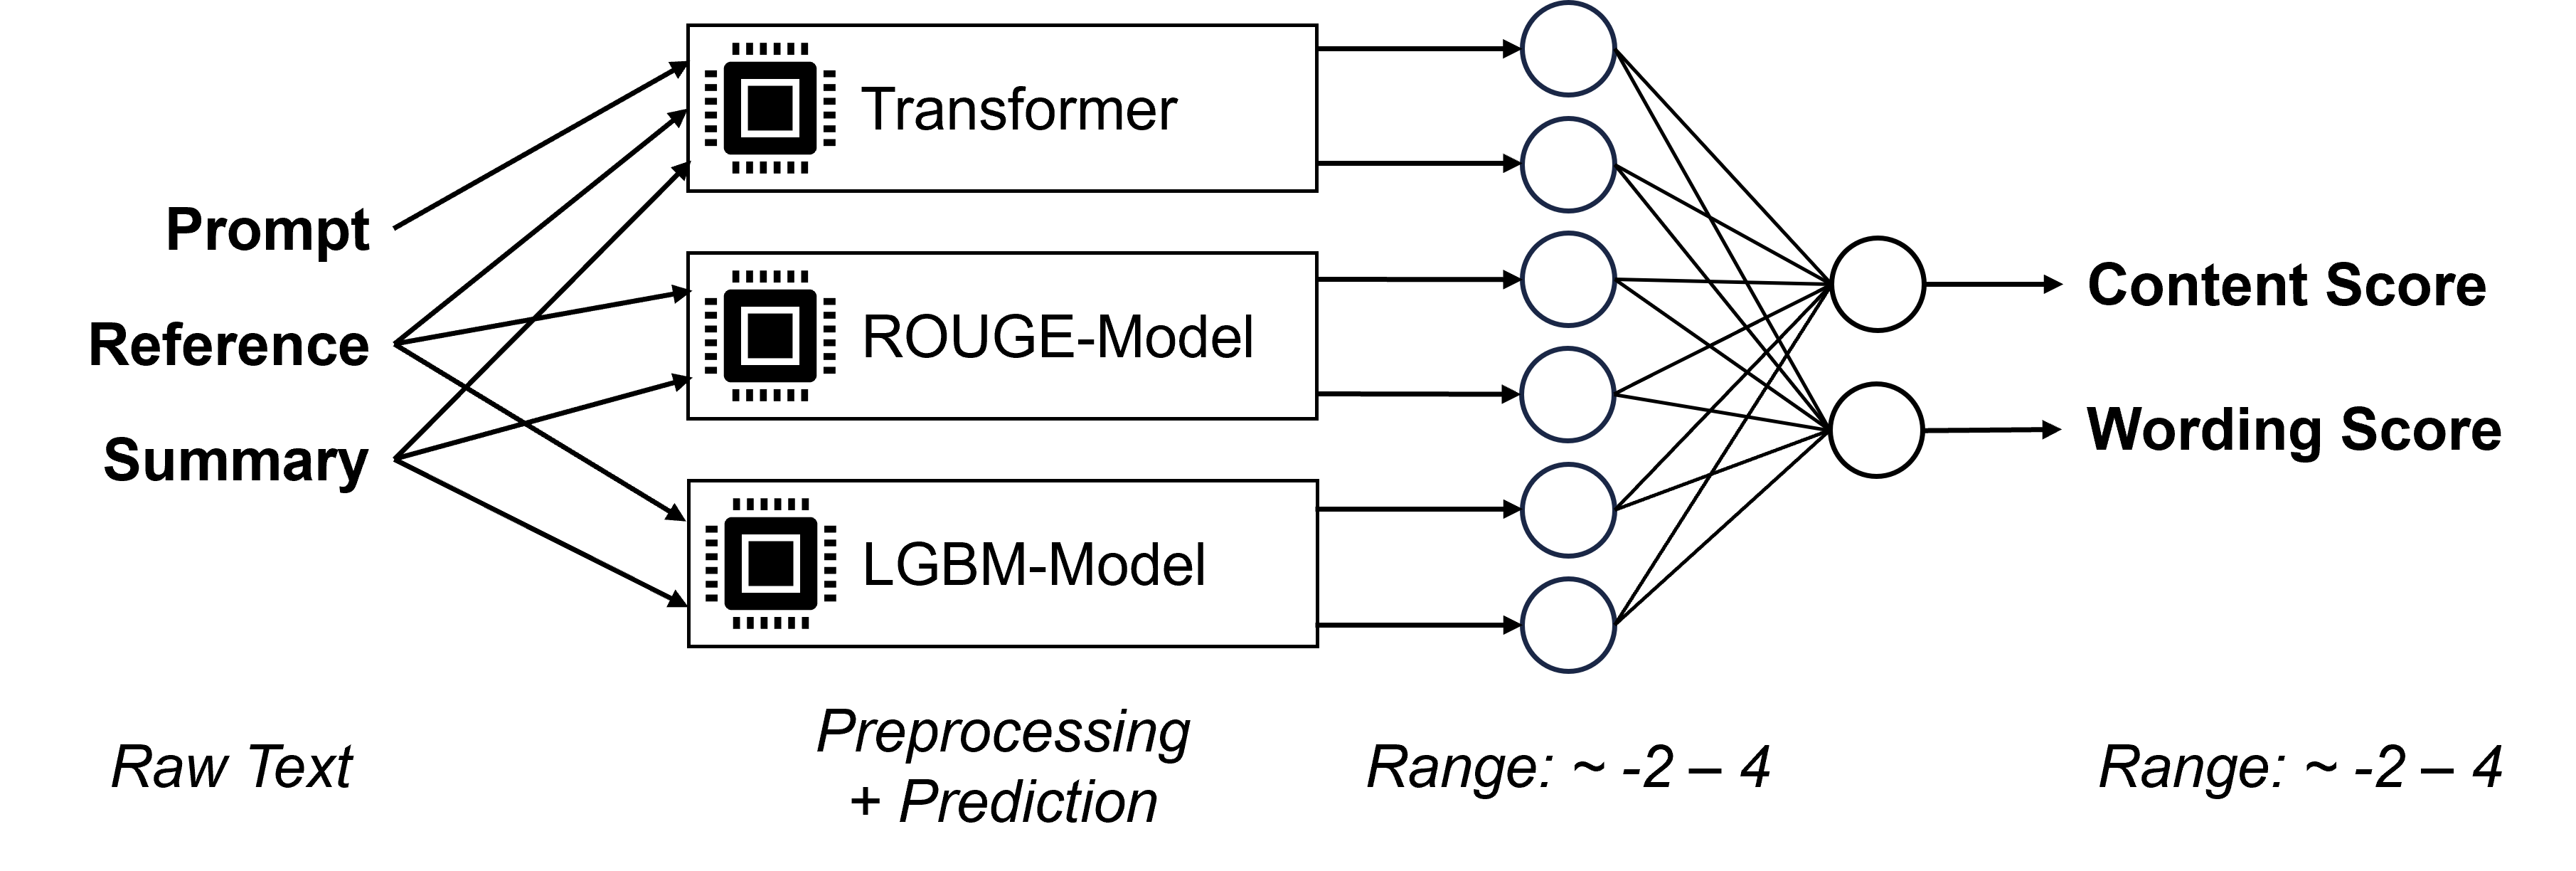
\includegraphics[keepaspectratio, width=\textwidth]{Ensemble-Model.png}
\caption{Architecture of the Ensemble-Model.}
\label{fig:ensemble-model}
\end{figure}

\subsubsection{Hyperparameter Tuning}

The "learned weighted average" approach was the only one investigated for this model. Since the model consists of just one linear layer, there were only a few parameters to test. While experimenting with hidden layers for this model, it became clear quite quickly that the added non-linearity, no matter the \gls{activation function}, reduced performance. However, like the ROUGE-Based Model, the simplicity meant that the Ensemble Model was robust against overfitting as well as changes to the \gls{lr} and the number of training \glspl{epoch}. Leading to the following hyperparameters:

\begin{itemize}
    \item \textbf{\glsdisp{hidden-layer}{Hidden-Layers}:} 0 Hidden Layers
    \item \textbf{\glsdisp{hidden-dim}{Hidden-Dim}:} 0 Neurons 
    \item \textbf{\glsdisp{activation function}{Activation Function}:} No Activation Function
    \item \textbf{\glsdisp{lr}{Learning Rate}:} 0.01
    \item \textbf{\glsdisp{epoch}{Epochs}:} 10 Epochs
\end{itemize}
